\chapter{Search for p-wave Annihilating DM with \Fermi-LAT}
\section{\Fermi-LAT Observations of the Galactic Center}\label{sec:GC}

{\it Fermi}-LAT is an all-sky pair-conversion telescope which has been successfully observing the $\gamma$-ray sky between a few tens of MeV to more than a TeV for ten years.
Incoming gamma rays pass through an anti-coincidence detector and convert in a tracker to $e^{+}/e^{-}$ pairs. 
Energy is deposited by the $e^{+}/e^{-}$ pairs in a NaI calorimeter.
The charged particle direction is reconstructed using the information in the tracker, and the energy is estimated from depositions in the calorimeter.  
Detailed descriptions of the LAT and its performance can be found in dedicated papers~\cite{Atwood:2009ez,2013arXiv1303.3514A}. 
In our data selection, {\it Fermi}-LAT has an integrated exposure of approximately $4.5 \times 10^{11}$ cm$^2$s in the direction of Sag A*.

\subsection{Data Selection}\label{sec:fermi}

For this analysis, we used nine years of LAT data (2008 August 4 to 2017 March 5) selecting {Pass 8} SOURCE-class events 
in the energy range from 6 GeV to 800 GeV, binned in 50 logarithmically-spaced energy bins and 0.04$^\circ$ angular pixelization. 
The energy range was chosen to avoid the well-known \cite[e.g.][]{GC2016} complexities of modeling the GC at energies of a few GeV. In addition,
the {\it Fermi}-LAT point-spread function (PSF) improves by nearly an order of magnitude between 1 GeV and 10 GeV, which improves its sensitivity to a signal that is localized as a point-like source.

We chose a small ROI which had a radius of 1$^\circ$, centered at Sag A* for two reasons: a) our putative DM signal is a point source spatially coincident with Sag A*, and the {\it Fermi} 95\% containment radius at 10 GeV is less than 1$^\circ$, so our ROI should contain virtually all of the signal, and b) our analysis relies mostly on searching for sharp spectral features, so contamination of unmodeled nearby point sources was not a particular concern.
We found the farthest point source from Sag A* in our ROI, 1FIG J1748.2-2816, had negligible correlation with the parameters of the Galactic center source.
In any case, the resulting model showed no indications that our ROI had any appreciable contamination from sources beyond 1$^\circ$ from Sag A*.

We modeled the performance of the LAT using the {P8R2\_SOURCE\_V6} Instrument Response Functions (IRFs).
The data processing and exposure calculations were performed using the LAT \textit{ScienceTools} version 
10-00-05\footnote{\url{http://fermi.gsfc.nasa.gov/ssc/data/analysis/software}}. 
A summary of the parameters of our data selection is available in Table \ref{tab:data2}, and a counts map of the data is shown in the left panel of Figure \ref{fig:roi_residmap}.

\begin{table}[ht]
\begin{tabular}{cc}
\hline \hline
Selection & Criteria \\ \hline
Mission Elapsed Time (s)\footnote{$Fermi$ Mission Elapsed Time is defined as seconds since 2001 January 1, 00:00:00 UTC} & 239557417 to 516826903  \\ 
Instrument Response Functions & P8R2\_SOURCE\_V6 \\
Energy Range (GeV) & 6-800 \\
Fit Region & 1$^\circ$ radius, centered on (RA, DEC)=(266.417, -29.0079) \\ 
Zenith Range & $\theta_z<$100$^\circ$ \\
Data Quality Cut with the $gtmktime$ Science Tool\footnote{Standard data quality selection: \texttt{DATA\_QUAL==1 $\&\&$ LAT\_CONFIG==1}} &  Yes \\ \hline
\end{tabular}
\caption{ \label{tab:data2} Data selection used by this paper's analysis }
\end{table}

\begin{figure}[ht] 
\begin{center}
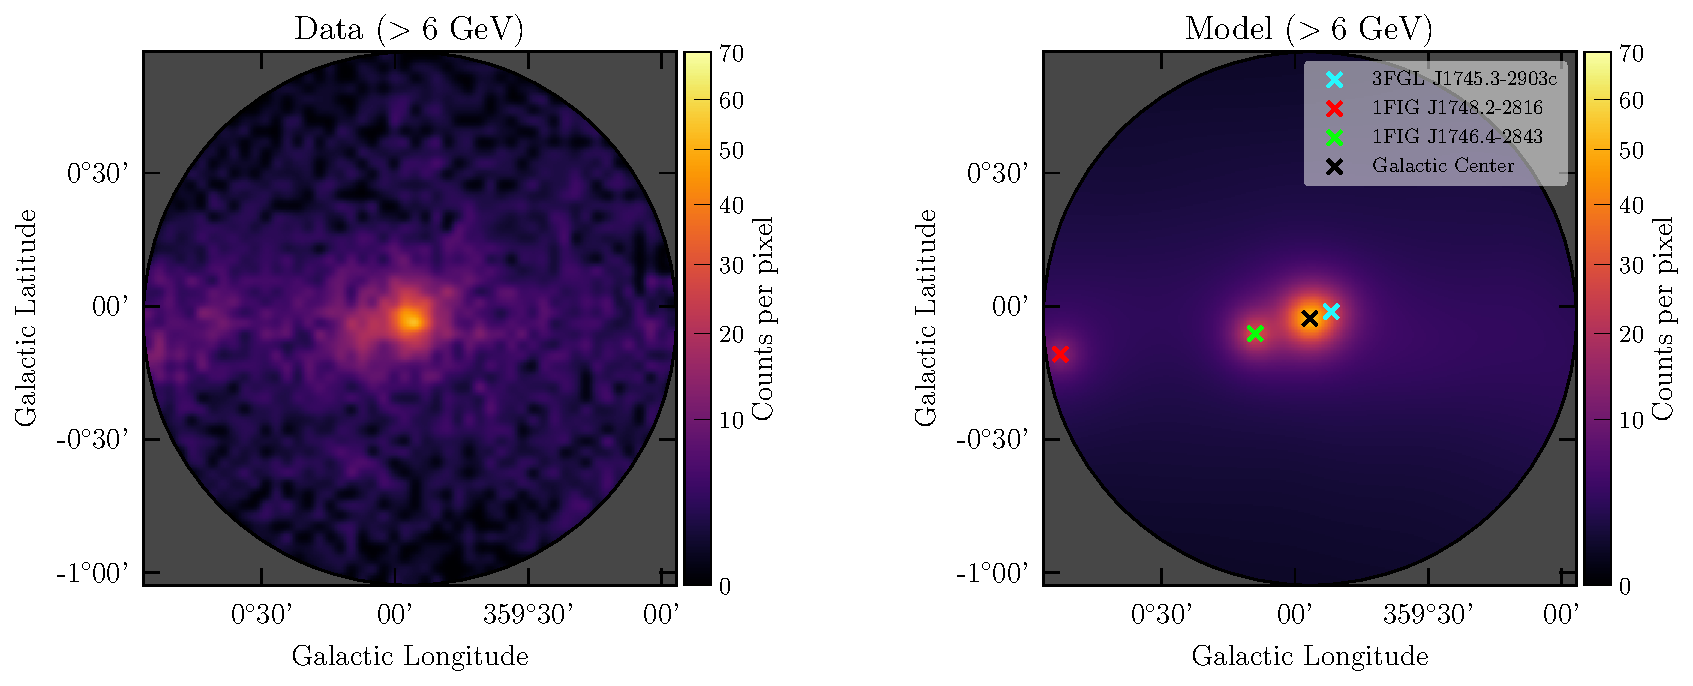
\includegraphics[width=0.9\columnwidth]{figures/dataModelComparison}
\noindent
\caption{ 
\label{fig:roi_residmap}
{\it Left panel:} Total photon counts in the ROI used in the analysis. The GC source is prominently seen near the center of the image, while the Galactic diffuse emission is responsible the majority of the photons outside the GC. {\it Right panel:} Model of the ROI after fitting with {{\tt gtlike}} (see Section \ref{sec:model_GC}), with the four point sources in the image labeled. In both maps, the pixel size is 0.04$^\circ$ and a Gaussian smoothing has been applied.
}
\end{center}
\end{figure}

\subsection{Modeling the Galactic Center}\label{sec:model_GC}

In order to search for a DM signal via the maximum-likelihood analysis described in Section \ref{sec:analysis}, we required a model of the ROI.
Our model was built from diffuse components and objects listed in the \textit{Fermi}-LAT Third Source Catalog (3FGL)~\cite{REF:2015.3FGL} and 1FIG~\cite{GC2016}. 

Once a model was defined, we compute its likelihood $\mathcal{L}(n,\theta)$ by:
\begin{equation}
\label{eq:likelihood}
\mathcal{L}(n, \theta) = \prod_{i=0}^{N}\frac{\mu_i^{n_i}}{n_i!}e^{-\mu_i}
\end{equation}
Where the index $i$ runs over the angular and energy bins, and $n$ is the actual data. 
We vary the model parameters $\theta$ until the likelihood is maximized; in practice we take the logarithm of the result. 
The likelihood computation and maximization was performed by the {\it Fermi} Science Tool \textup{gtlike}, which in turn used the MINUIT \cite{MINUIT} optimization routine.

\subsubsection{Diffuse Components and Extended Sources}\label{sec:diffuse}
Although a custom interstellar emission model (IEM) was successfully used to model the GC in previous works~\cite{GC2016} based on the Pass 7 data reconstruction, generating a similar custom IEM for the Pass 8 data used here was deemed to be outside the scope of this paper; the diffuse components used in this analysis were the standard Pass 8 models taken from the Fermi Science Support Center\footnote{The diffuse background models are available at: \url{http://fermi.gsfc.nasa.gov/ssc/data/access/lat/BackgroundModels.html} as {is\_P8R2\_SOURCE\_V6\_v06.txt} and {gll\_iem\_v06.fits}.}.
After fitting the data we found that the contribution of the isotropic component of our model was negligible when compared to the Galactic diffuse component; we decided not to include an isotropic component in the final model for this reason.

\subsubsection{Point Sources}
There are two point source catalogs that are relevant for our ROI: the 3FGL and 1FIG.
However, because our analysis covers a different time and energy range than either of the catalogs, it was not expected that either catalog would fit the data perfectly.
Instead, each catalog (along with the diffuse component from Section \ref{sec:diffuse} above) was used to fit the data separately, and sources that were insignificant above 10 GeV were excluded.
The three remaining sources were then used together to form our final model, which was found to yield better results than the results of each catalog individually.
For simplicity, we used a power law to describe the spectrum of all the sources in the model; none of the sources were fit significantly better by a curved spectrum over the energy range considered.

The GC is the most complicated region of the $\gamma$-ray sky, and as a result the point source associated with Sag A* is flagged in the 3FGL catalog as strongly dependent on the model of Galactic diffuse emission. 
However, a complete study of different diffuse emission models and their effects on the GC source properties was deemed outside the scope of this work, for which we needed only an empirical model against which we can test our DM hypothesis.

We found when fitting our data that the GC source was better fit by a narrow Gaussian distribution than a simple point source:
\begin{equation}
\rho (r) = \frac{1}{\sqrt{2\pi\sigma_r^2}}\exp{\frac{-r^2}{2\sigma_r^2}}
\end{equation}

with $\sigma_{r}=0.03^\circ$, and $r$ measured in degrees.
Although $\sigma$ is smaller than the {\it Fermi}-LAT PSF at 10 GeV, the extension was found to improve the residuals between the model and data, especially at the particular location of Sag A*- see Figure \ref{fig:residmapComparison}. 


\begin{figure}[ht] 
\begin{center}
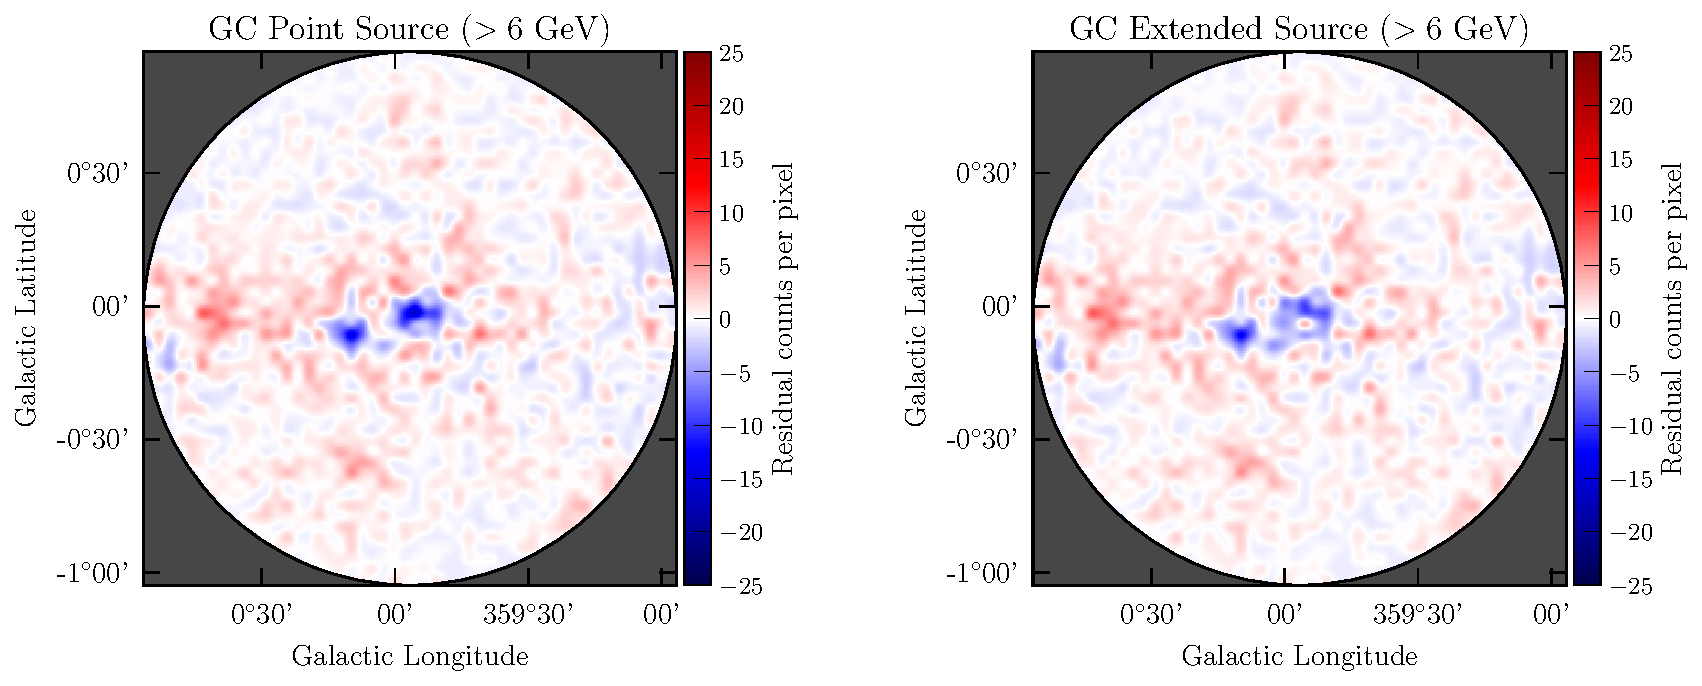
\includegraphics[width=0.9\columnwidth]{figures/residComparison.pdf}
\noindent
\caption{ 
\label{fig:residmapComparison}
{\it Left Panel}: The counts residuals for the best-fit model using a point source description of the Galactic Center source.
{\it Right Panel}: Residuals given a slightly extended source as described in the text, showing modest improvement at the location of Sag A. In both panels the angular pixelization and smoothing are the same as in Figure \ref{fig:roi_residmap}}
\end{center}
\end{figure}

A summary of the sources used in the model is shown in Table \ref{tab:model}, and the best-fit model (integrated over the energy range) is shown in the right panel of Figure \ref{fig:dataModelComparison}.

\begin{table}[ht]
\begin{tabularx}{\textwidth}{c @{\extracolsep{\fill}} ccccc}
\hline \hline
Source Description & Spectral Model & $N_{\gamma}$ & Spatial Model & RA & DEC\\ \hline
Galactic diffuse emission & PowerLaw & 4397 & MapCube & - & - \\ 
GC & PowerLaw & 1337 & Gaussian distribution, $\sigma = 0.03^{\circ}$ & 266.42 & -29.01 \\
1FIG J1746.4-2843 & PowerLaw & 536 & Point Source & 266.59 & -28.86 \\
1FIG J1748.2-2816 & PowerLaw & 176 & Point Source & 267.10 & -28.28 \\
3FGL J1745.3-2903c & PowerLaw & 169 & Point Source & 266.34 & -29.06 \\
\hline
\end{tabularx}
\caption{ \label{tab:model} List of sources used in modeling the ROI. }
\end{table}

As a check of our systematic uncertainty, we also performed the following analysis using a separate dataset covering 4 years of data with Pass 7 data reconstruction.
The model of the ROI contained the same point sources as presented here, however the diffuse models were the custom Pass 7 models from the work in \citep{GC2016}. 
The resulting flux upper limits were found to be consistent with the main analysis presented below- for simplicity we present only the standard analysis with Pass 8 data reconstruction.

%In the most conservative possible model, one could remove the GC source and consider all the flux from the Galactic Center as originating from DM annihilation.
%Although we do not regard this model as physically realistic, we analyzed this case separately and found the resulting upper limits on the annihilation flux to be about a factor of $10^2$ greater across the energy range considered.

\section{Analysis}\label{sec:analysis}


\subsection{Fitting Method}\label{sec:fitting}
As discussed in Section \ref{sec:dm}, the phenomenology of our reference model p-wave DM signal is that of a point source located at the location of Sag A*, with an energy spectrum that is flat between two endpoints (a `box' shape).
For this analysis, we considered two representative versions of the box: the `wide' box has a value of $\zeta = 0.44$, while the `narrow' box has a value of $\zeta = 0.9999$.
Implications from the two types of searches for mass splittings in intermediate cases are discussed in Section \ref{sec:conclusion}.

We searched for $\gamma$-ray boxes which had an upper-edge energy equal to the boundaries of the energy bins between 10 and 658 GeV in our data selection, corresponding to 42 different DM hypotheses.
In order to prevent edge effects from impacting the results, boxes with upper edges outside of this range were not considered. 
An example DM signal (integrated over the ROI), along with the background, is shown in the left panel of Figure \ref{fig:artificial_box}. 

The significance of each DM hypothesis was evaluated using the test statistic (TS) defined as: 
\begin{equation}
\mathrm{TS}=2~\mathrm{ln}\frac{\mathcal{L}(\mu, \theta | \mathcal{D})}{\mathcal{L}_{\mathrm{null}}(\theta | \mathcal{D})} \label{eq:ts}
\end{equation}
Where $\mu$ is the signal strength, $\theta$ is the array of parameters describing the DM hypothesis (in this case, the energy and width of the $\gamma$-ray box, and $\mathcal{D}$ represents the binned data. $\mathcal{L}_{\mathrm{null}}$ is the value of the likelihood in the absence of any signal.
The likelihood values $\mathcal{L}$ are computed from Equation \ref{eq:likelihood}.

The TS value was then used to calculate a level of significance $Z$ via:
\begin{equation}
Z = \Phi ^{-1} \left( 1-\int_\mathrm{TS}^\infty \chi^2(x,k)dx\right)
\end{equation}
Where $\Phi ^{-1}$ is the inverse quantile function; the integral in this expression is the $p$-value.
Simulations (described below) confirmed that the TS values were distributed following a $\chi^2$ distribution with 1 degree of freedom (the total flux contained in the `box' signal)- see the left panel of Figure \ref{fig:correlations}. As the counts per bin decreases, the $\chi^{2}$ distribution moderately over-predicts the number of high TS trials observed in simulated data. 

The procedure for finding the TS of a given DM hypothesis and upper limit on the total flux of a $\gamma$-ray box with an upper edge at a particular bin energy was as follows:
\begin{enumerate}\label{sec:procedure}
\item \label{step:fit} The parameters of the model described in Section \ref{sec:model_GC} allowed to vary to maximize the likelihood function $\mathcal{L}$, giving the null likelihood.
This step was performed once for each set of 42 DM hypotheses that corresponded to the dataset under investigation (either the actual data or the Poisson fluctuations described below). 
\item The expected spectrum of the DM signal is calculated by convolving a ideal box spectrum with a Gaussian distribution representing with the \Fermi-LAT energy resolution, which is between 5\% and 10\% in the energy range considered. 
\item A point-source with the convolved DM spectrum is added to the model at the location of Sag A*, with a single overall normalization parameter $N$.
\item All parameters in the model except for the normalization of the central GC source are fixed.
A study of the correlation coefficients (see Section \ref{sec:correlations}) showed that the signal was modestly correlated with this source, but had negligible correlation with other parameters in the model.
Fixing the other parameters has the benefit of decreasing the computation time and preventing numerical instabilities when fitting a system with a large number of degrees of freedom.
\item The normalization $N$ of the DM source is increased from a value of 0 until the TS exceeds 2.71, which corresponds to a 95\% confidence upper limit on $N$, or a $Z$ value of approximately 2. The value of $N$ for which $\mathcal{L}$ is maximized and the corresponding TS are also stored in order to evaluate the significance of the best-fit DM hypothesis.
\end{enumerate}



\subsection{Correlations Between Background and Signal Components}\label{sec:correlations}

In order to understand the relationship between a potential signal and the background sources, we calculated the correlation coefficients between the signal source and the GC source.
As expected, both $\zeta=0.9999$ and $\zeta=0.44$ hypotheses are negatively correlated with the normalization of the GC background source.
We found that the signal became less correlated as the right edge of the box increases in energy, since the likelihood fit is strongly driven by the higher statistics at low energy.
We also found that the $\zeta=0.44$ hypothesis had a stronger correlation to the background when compared to the  $\zeta=0.9999$ case, which is expected because the $\zeta=0.44$ signal contributes over a broader energy range. 

A plot of the correlation coefficients in both cases as a function of the energy of the right edge of the box is shown in the right panel of Figure \ref{fig:correlations} below.
Because the GC source has a power-law spectral shape, its prefactor and index were found to be almost perfectly anticorrelated (correlation coefficient $<$-0.95), and therefore the correlation coefficient between the signal and GC index was nearly identical to that between the signal and GC prefactor.
We found that the correlation coefficients of the signal to the parameters of other sources in the model were negligible.

\begin{figure}[ht] 
\begin{center}
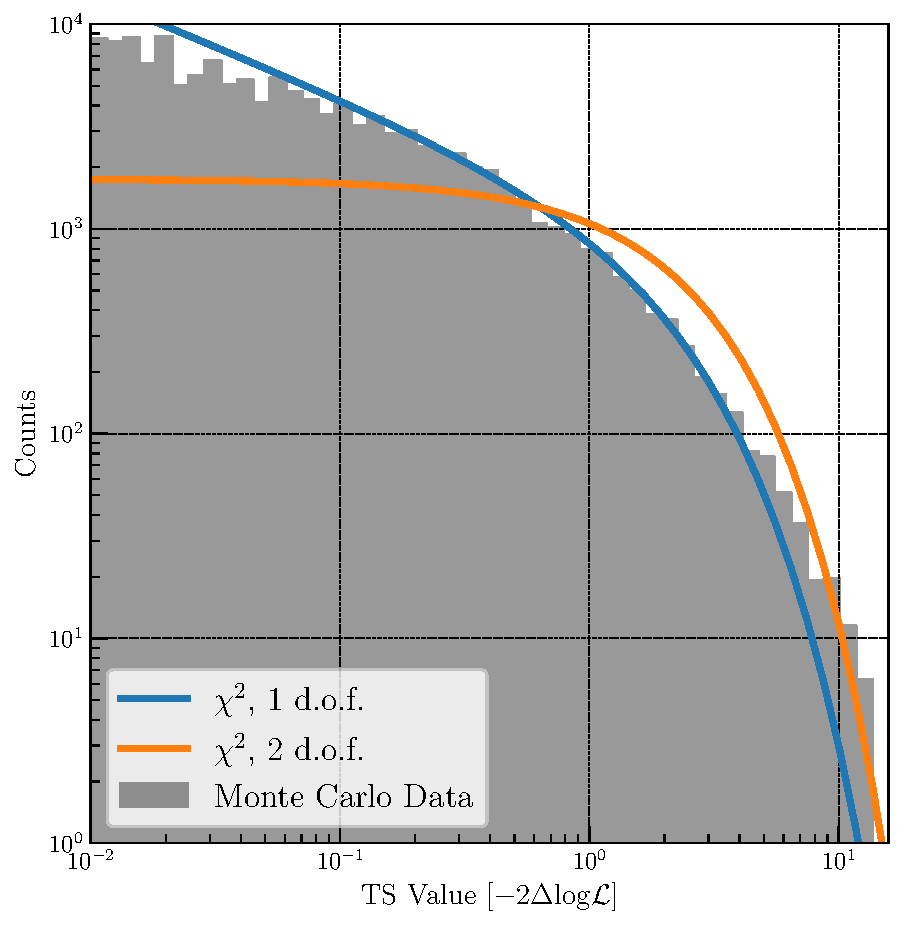
\includegraphics[width=0.45\columnwidth]{figures/ts_hist.pdf}
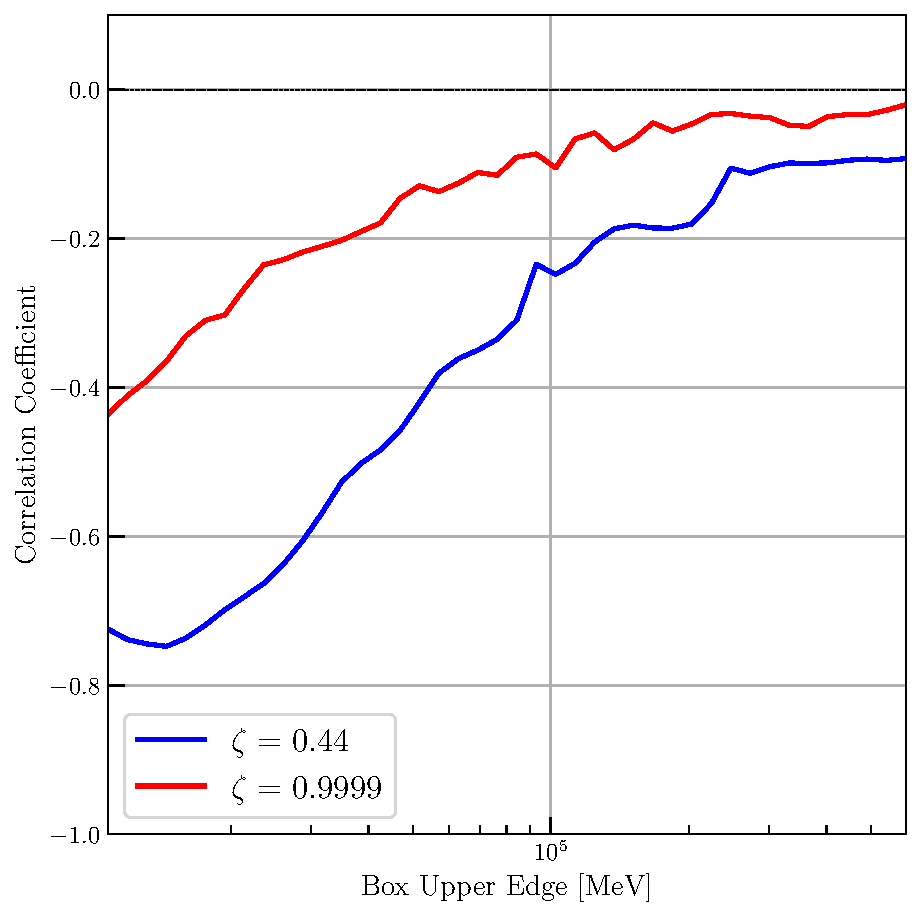
\includegraphics[width=0.45\columnwidth]{figures/correlation_coefficients.pdf}
\noindent
\caption{ 
\label{fig:correlations}
{\it Left Panel}: Histogram of TS values for all DM signal hypotheses from the Monte Carlo study for a $\zeta=0.44$ signal. The shape of the TS distribution is best-fit by a $\chi^2$ distribution with only one degree of freedom, although the $\chi^2$ distribution slightly underpredicts the true distribution at high TS. At the critical value of 2.71, the shape of the distribution is particularly well-described by the $\chi^2$ distribution. 
{\it Right Panel}: Correlation coefficients between the total flux of the DM signal hypotheses and the normalization $N$ of the GC source (modeled here as a power law, i.e. $\frac{dN}{dE} = Ne^{-\alpha E}$.
We evaluate the correlation as a function of the upper edge of the DM signal box, and find that the correlation is negligible for high-energy boxes but is becomes significant at lower energies because of the increased statistics in the data.
Because the two sources are spatially coincident, the sources are expected to be anticorrelated.
}
\end{center}
\end{figure}

\subsection{Monte Carlo Simulations\label{sec:MCMethods}}
We performed a Monte Carlo study in order to understand the impact that statistical fluctuations have on the analysis. 
Each instance of the Monte Carlo began by generating Poissonian fluctuations about the best-fit model of the data.
We then used the Poisson data as the input to the protocol defined in Section \ref{sec:fitting}, and stored both the upper limit and TS values for each DM hypothesis.
Because Step \ref{step:fit} above fits the parameters of the background model, this technique probes the effects of statistical uncertainty on both the signal and the background.
We performed O($10^3$) simulations, and used the upper limit curves from each instance to generate 68\% and 95\% containment bands in the cases of $\zeta = 0.44$ and $\zeta = 0.9999$.
The upper limits from the data and the containment bands from the Monte Carlo study are displayed in Figure \ref{fig:brazil_lines}.

\subsection{Reconstruction of Injected Signal\label{sec:injected}}
To confirm that the upper limit calculation was sensitive to the presence of a DM signal, and to understand how a signal would appear in our analysis, we injected a DM signal into the data and repeated the analysis procedure from Section \ref{sec:procedure}.
The injected DM signal for this test was defined to have $\zeta = 0.44$ and a total flux of $3.0*10^{-10} $ph cm$^{-2} $s$^{-1}$, with an upper energy endpoint of 100 GeV.
At 100 GeV, the ratio of the injected signal flux to the total flux in the ROI was about 30\%.
We performed the same Monte Carlo study on the injected-signal dataset to produce containment bands for the limit.

The results of the analysis are in good agreement with the known injected signal.
The best-fit DM hypothesis was found to have an upper edge energy of 102 GeV, and the reconstructed flux of the signal was $3.7*10^{-10}$ ph cm$^{-2} $s$^{-1}$; moreover, the signal was highly significant (TS=167).
The upper limit curve was found to contain a prominent bump near 100 GeV which noticeably exceeded the 68\% and 95\% containment bands from the Monte Carlo study, as seen in Figure \ref{fig:artificial_box}.
%The upper limit at 100 GeV was $4.5*10^{-10}$ ph cm$^{-2} $s$^{-1}$.  
We concluded that the analysis procedure defined in Section \ref{sec:fitting} is sensitive to the presence of a realistic DM signal, and can accurately reconstruct its parameters.
The best-fit box is shown in the left panel of Figure \ref{fig:artificial_box}.


\begin{figure}[ht]
\begin{center}
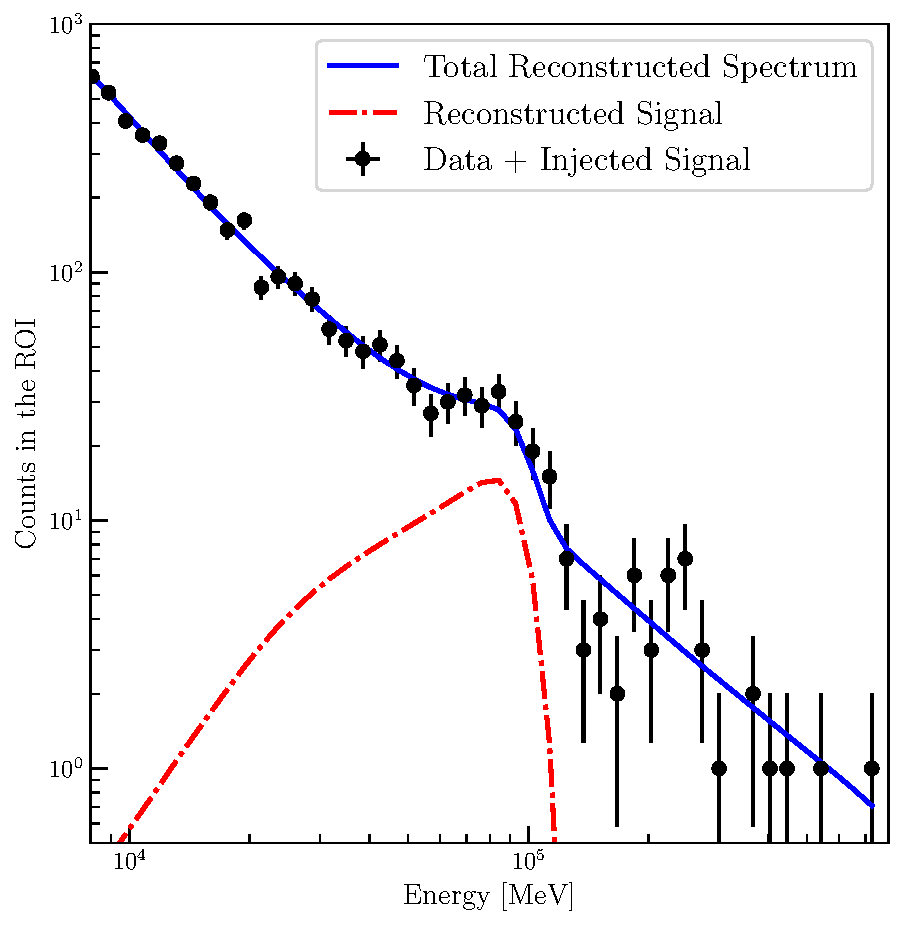
\includegraphics[width=0.45\columnwidth]{./figures/good_box_fit.pdf}
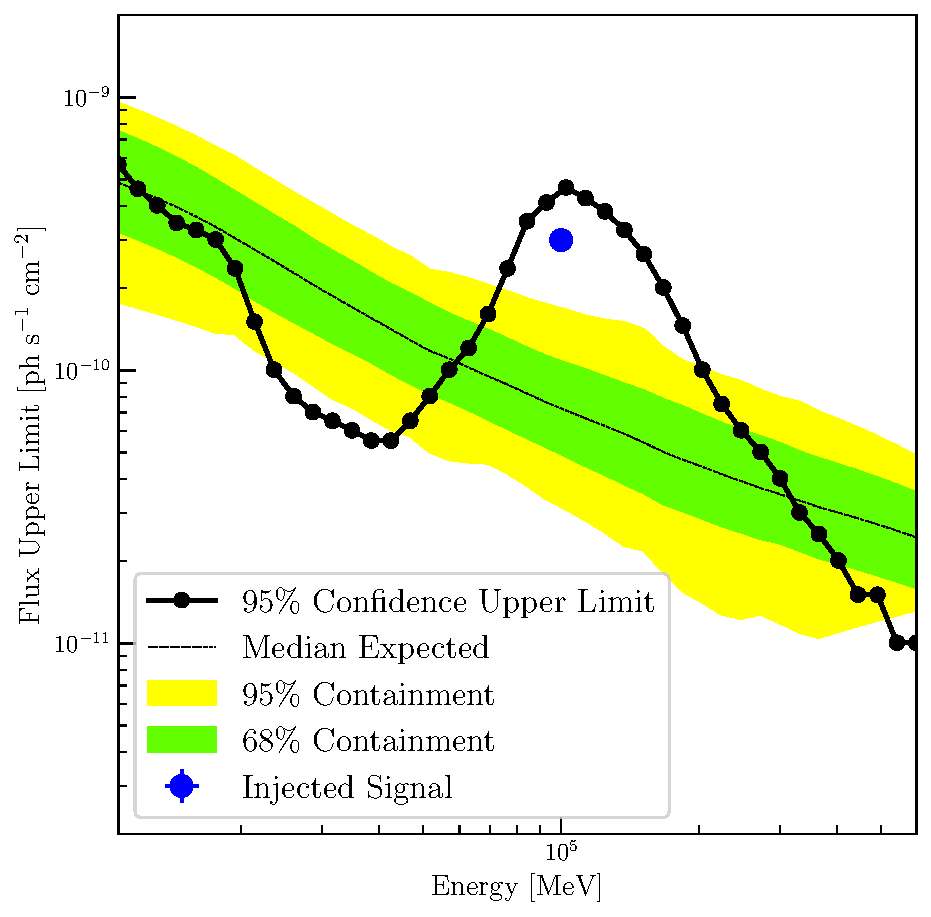
\includegraphics[width=0.45\columnwidth]{./figures/brazil_artificial_box.pdf}
\noindent
\caption{
\label{fig:artificial_box}
{\it Left Panel}: Energy spectrum of the data + injected signal. The 'box' DM signal appears as a prominent bump near its upper endpoint. 
{\it Right Panel}: The DM signal upper limit (in black) in the presence of an injected box with upper endpoint 100 GeV and total flux $3*10^{-11} $ ph cm$^{-2} $s$^{-1}$. The blue dot shows the position of the injected signal.
The 68\% and 95\% containment bands are constructed from performing the analysis on Poisson-fluctuated datasets about the best-fit background model. 
Our injected DM signal is not excluded by the analysis. 
}
\end{center}
\end{figure}


\section{Results}\label{sec:results}

No significant signal from a p-wave DM signal was seen in either the case of the wide or narrow box.
The flux upper limits are shown in Figure~\ref{fig:brazil_narrow_box} for both the wide box (left panel) and the narrow box (right panel) scenarios. 
The strongest signal came in the case of $\zeta = 0.9999$ at energy 247 GeV; the TS of this DM hypothesis was 4.0, corresponding to a local significance of 1.7$\sigma$ with one degree of freedom.
In the case of $\zeta = 0.44$, the strongest signal came from a box with an upper-edge energy of 17 GeV; the TS of the signal was 3.5 for a significance of 1.5$\sigma$.
These do not take into account trials factors, so their global significance is reduced further.

\begin{figure}[ht] 
\begin{center}
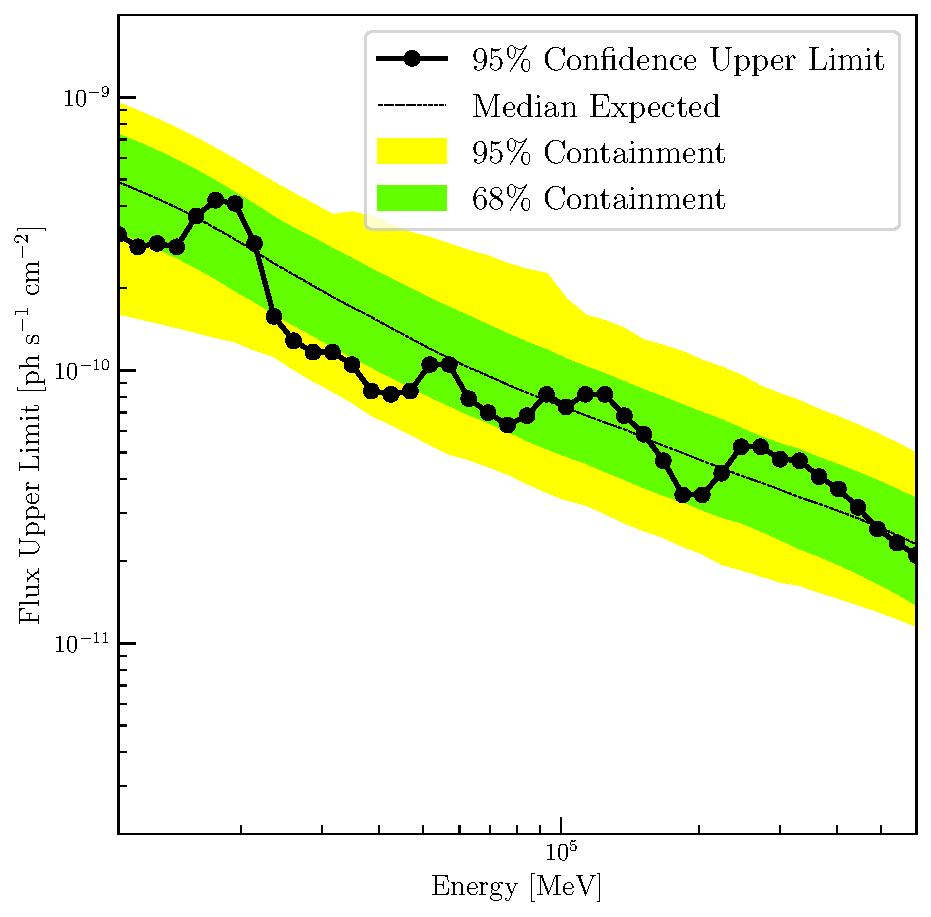
\includegraphics[width=0.45\columnwidth]{figures/brazil_wide_box.pdf}
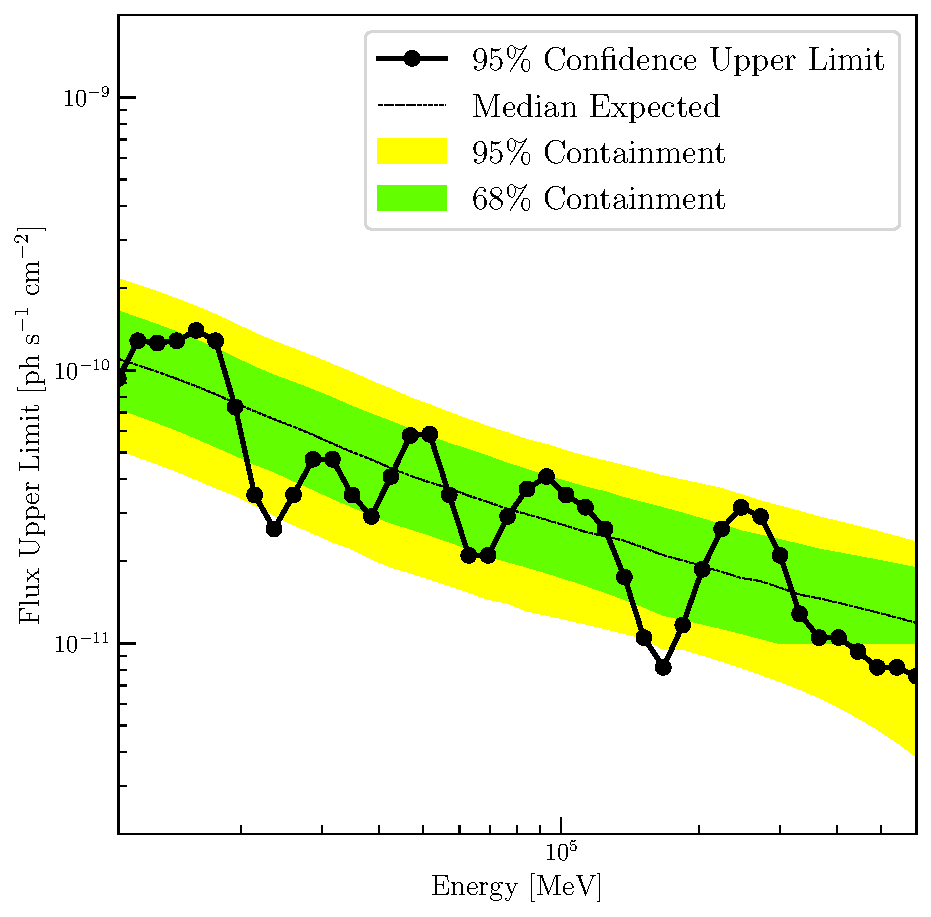
\includegraphics[width=0.45\columnwidth]{figures/brazil_narrow_box.pdf}
\noindent
\caption{ 
\label{fig:brazil_lines}
95\% confidence flux upper limit on a $\gamma$-ray box point source at the GC. In the left figure, the box extends from 0 GeV to the energy indicated (wide box). On the right, the width of the box is 1 GeV (narrow box). The 68\% and 95\% containment bands come from a Monte Carlo simulation of the data described in Section \ref{sec:MCMethods}. \label{fig:brazil_narrow_box}
}
\end{center}
\end{figure}

%\begin{figure}[ht] 
%\begin{center}
%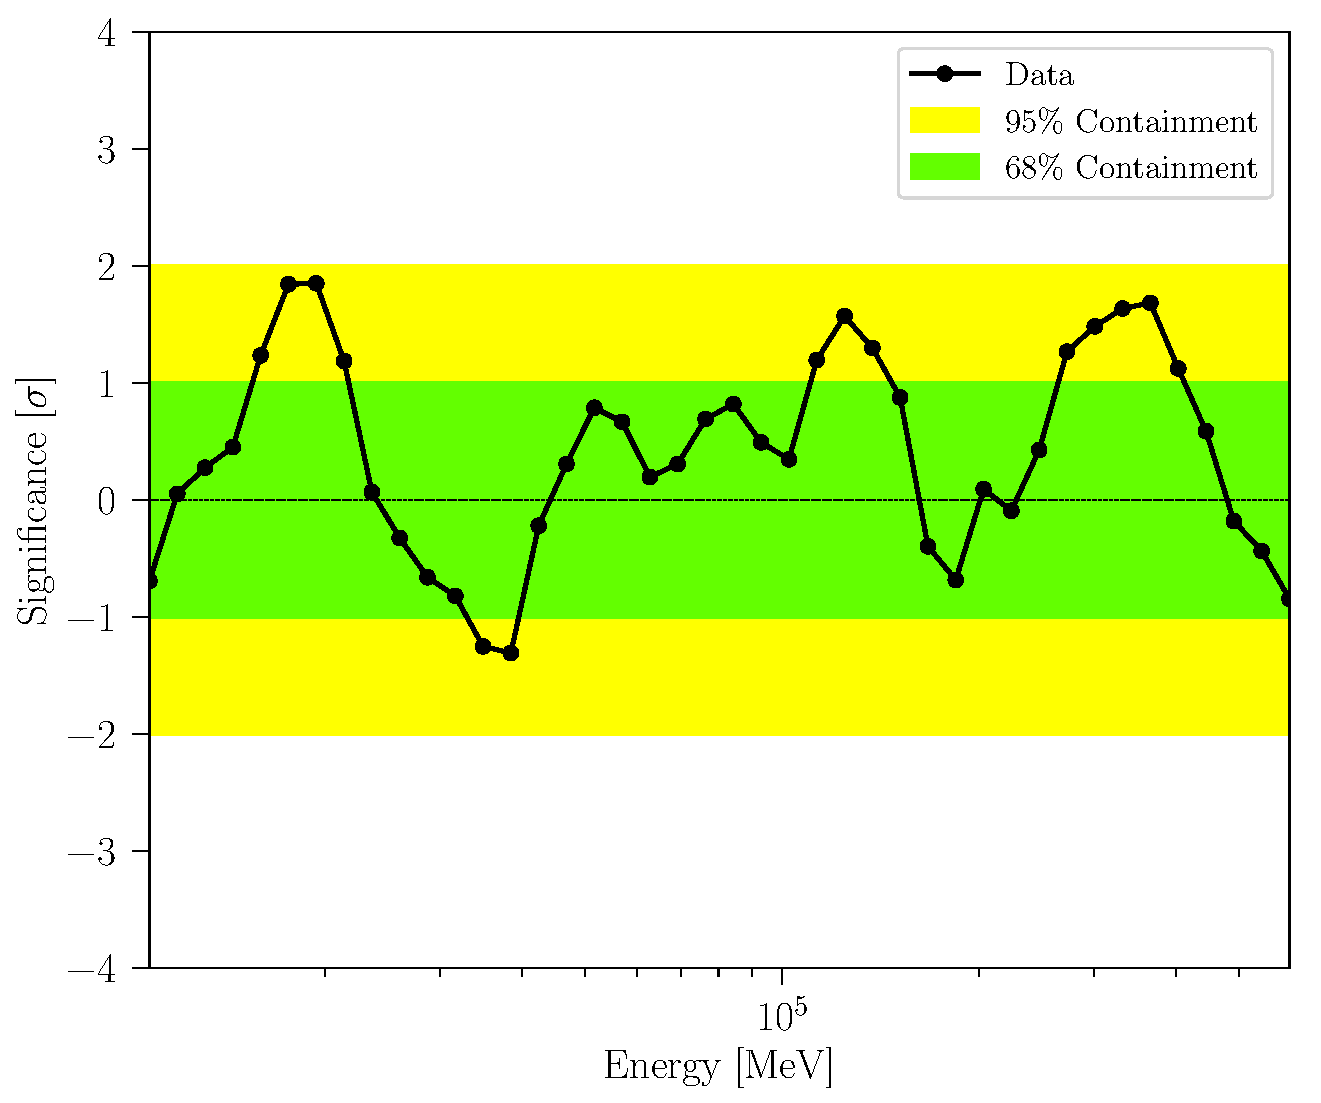
\includegraphics[width=0.45\columnwidth]{figures/significance_wide_box.pdf}
%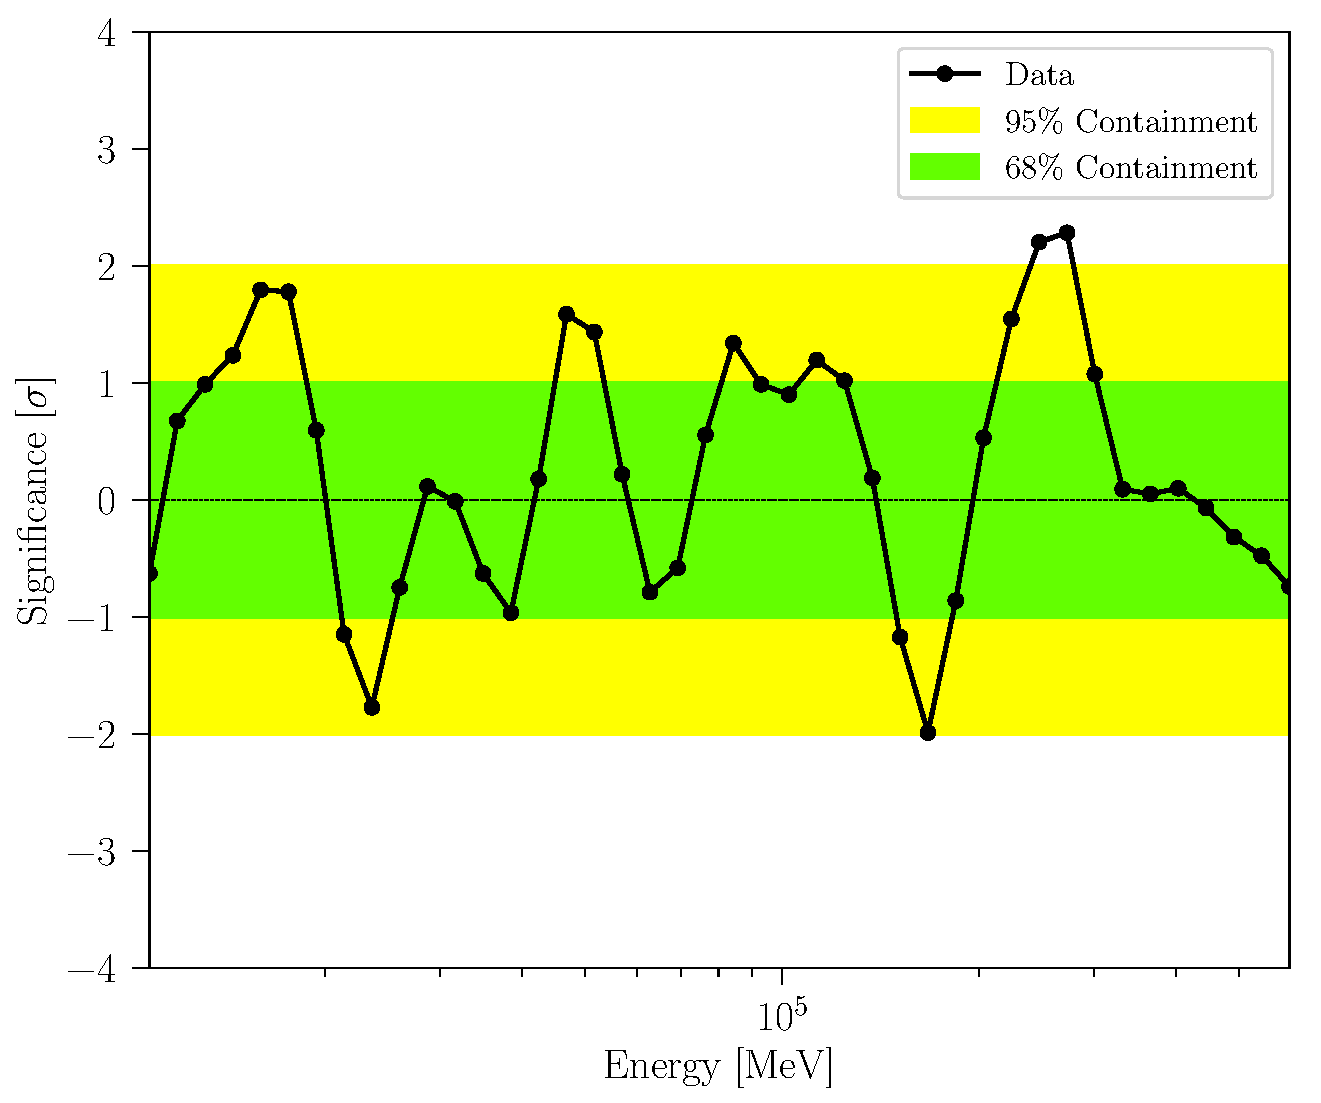
\includegraphics[width=0.45\columnwidth]{figures/significance_narrow_box.pdf}
%\noindent
%\caption{ 
%\label{fig:significances}
%The significance curves for the wide box case on the left, and the narrow box case on the right. In both cases the most significant bump occurs at around 16 GeV; the bump has a local significance of 2.3$\sigma$ in the wide-box case and a local significance of 2.9$\sigma$ in the narrow-box case. The global significances are 0.3$\sigma$ and 1.4$\sigma$, respectively.
%}
%\end{center}
%\end{figure}

The predicted flux from $p$-wave DM annihilation depends on the DM mass $m_{DM}$ as well as on the power laws of the DM halo ($\gamma_c$) and spike ($\gamma_{sp}$) in our fiducial model.  In Figure~\ref{fig:final_interp} we fix the DM mass, and show how the upper limits on narrow and wide boxes constrain the allowed DM distribution in the GC.  We can observe in particular that adiabatic spikes are excluded for even very shallow cusps $\gamma_c = 0.8$.  In this parameter space, DM models yielding narrow boxes are less constrained than DM models yielding wide boxes, despite the stronger flux limits; this occurs because the limited phase space available for the narrow box annihilation process further suppresses the annihilation.




\begin{figure}[ht] 
\begin{center}
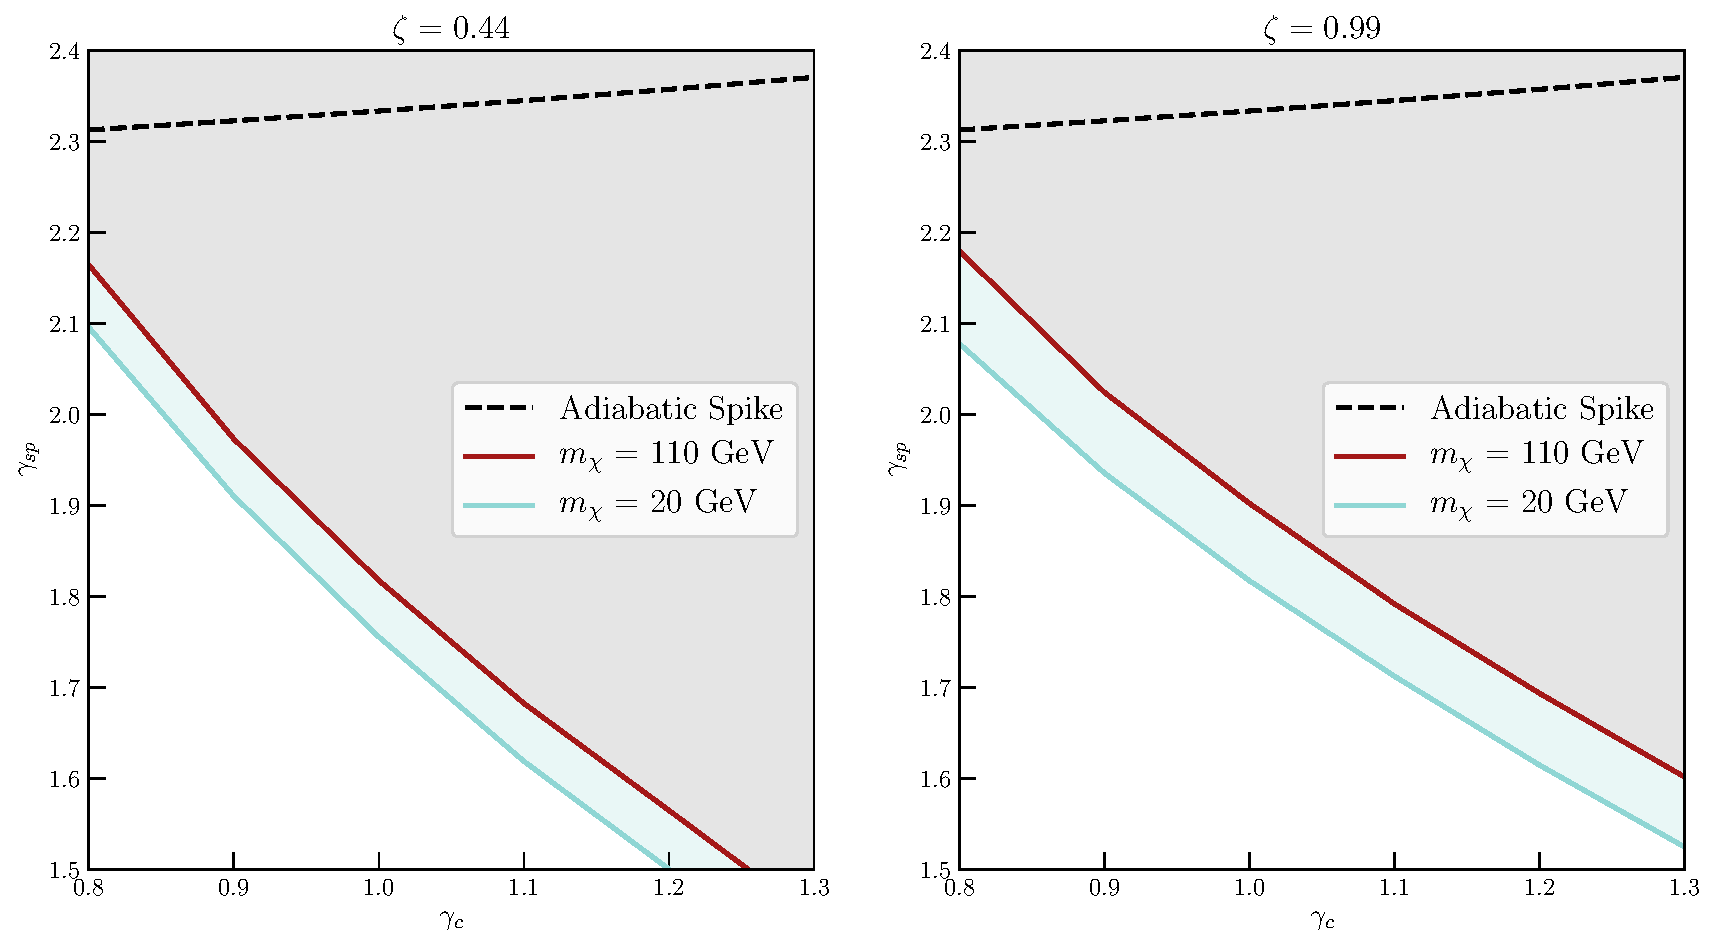
\includegraphics[width=0.9\columnwidth]{figures/final_interpretation.pdf}
\noindent
\caption{ 
\label{fig:final_interp}
DM distributions in the GC compatible with thermal relic $p$-wave DM in the hidden sector axion portal model, shown for two representative choices of DM mass $m_\chi = 20$ GeV, 110 GeV for narrow boxes (left, $\zeta=0.99$) and wide boxes (right, $\zeta = 0.44$).
}
\end{center}
\end{figure}

In Figure~\ref{fig:near-final} we consider fixed sample choices of $\gamma_c$ and $\gamma_{sp}$ and show the resulting limits on our reference hidden sector axion portal $p$-wave DM model as a function of DM mass.  For clarity we plot the ratio of the excluded cross-section $\langle\sigma v\rangle$ to the value of the cross-section that yields the correct relic abundance, $\langle\sigma v\rangle_{\mathrm{thermal}}$.  We comment that exclusions for the narrow box scenario in this reference model should not be considered literally at high masses as the model becomes non-perturbative above $m_\chi\sim 300$ GeV.  The need for such large couplings arises to compensate for the phase space suppression that follows when $m_\chi\approx m_\phi$, and no such issue arises in the wide box scenario.


\begin{figure}[ht] 
\begin{center}
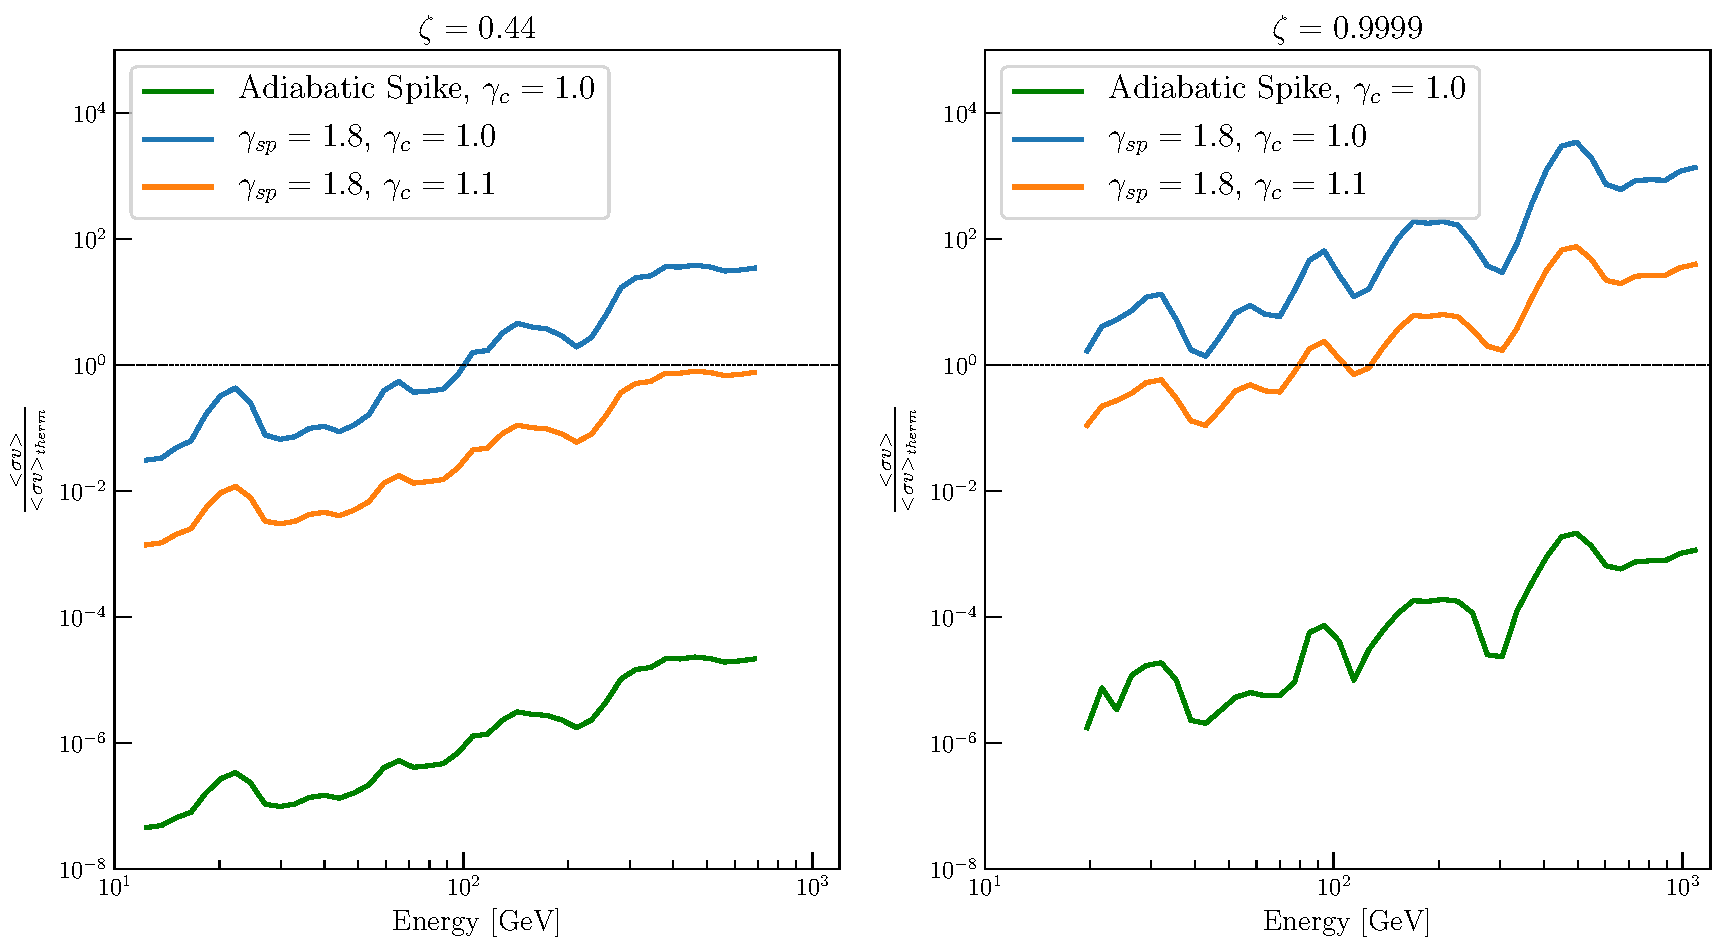
\includegraphics[width=0.9\columnwidth]{figures/final_fixed_astro.pdf}
\noindent
\caption{ 
\label{fig:near-final}
Limits on DM annihilation cross-section as a function of DM mass for fixed values of $\gamma_c$, $\gamma_{sp}$.   For clarity we plot the velocity-independent ratio of the excluded cross-section to the value that yields the correct relic abundance.  From top to bottom, the three curves correspond to  $\gamma_c = 1.1, \gamma_{sp}=1.8$ (orange);  $\gamma_c = 1.0, \gamma_{sp}=1.8$ (blue); and $\gamma_c = 1, \gamma_{sp}=2.33$ (adiabatic spike, green).
}
\end{center}
\end{figure}
